%%%%%%%%%%%%%%%%%%%%%%%%%%%%%%%%%%%%%%%%%%%%%%%%%%%%%%%%%%%%%%%%%%%%%%%%%%%%%%%%
%2345678901234567890123456789012345678901234567890123456789012345678901234567890
%        1         2         3         4         5         6         7         8

\documentclass[letterpaper, 10 pt, conference]{IEEEconf}  % Comment this line out
                                                          % if you need a4paper
%\documentclass[a4paper, 10pt, conference]{ieeeconf}      % Use this line for a4
                                                          % paper

% See the \addtolength command later in the file to balance the column lengths
% on the last page of the document
\usepackage[table,xcdraw]{xcolor}
\usepackage{amsmath,amsthm,amssymb}
\usepackage{float}
\usepackage[pdftex]{graphicx}
\usepackage{graphicx}
\usepackage{color}
\usepackage{mathtools}          %loads amsmath as well
\usepackage{titlesec}

\titlespacing\section{0pt}{12pt plus 4pt minus 2pt}{0pt plus 2pt minus 2pt}
\titlespacing\subsection{0pt}{12pt plus 4pt minus 2pt}{0pt plus 2pt minus 2pt}
\titlespacing\subsubsection{0pt}{12pt plus 4pt minus 2pt}{0pt plus 2pt minus 2pt}

% The following packages can be found on http:\\www.ctan.org
%\usepackage{graphics} % for pdf, bitmapped graphics files
%\usepackage{epsfig} % for postscript graphics files
%\usepackage{mathptmx} % assumes new font selection scheme installed
%\usepackage{times} % assumes new font selection scheme installed
%\usepackage{amsmath} % assumes amsmath package installed
%\usepackage{amssymb}  % assumes amsmath package installed

\title{\LARGE \bf Cruise Control: A HLS Design Tool for Low Power Systems}
\author{Andrew Smith(atsmith3) and Thomas Furlong(tfurlon2)}% <-this % stops a space

\begin{document}

\maketitle
\thispagestyle{empty}
\pagestyle{empty}


%%%%%%%%%%%%%%%%%%%%%%%%%%%%%%%%%%%%%%%%%%%%%%%%%%%%%%%%%%%%%%%%%%%%%%%%%%%%%%%%
\section{Abstract}
Vivado High Level Synthesis (HLS) has been proven to be a great tool for the rapid prototyping, development, and optimization of hardware accelerators and IP's. The tools within HLS allow developers to move away from low level hardware description languages and use higher, system level languages such as C and C++. By moving away from the hardware languages, projects developed in HLS have a quicker time to market. While developing in HLS, the optimization that users can place are all done manually. Developers must have an understanding of the different optimization pragmas and how to place them in the code. Once the pragmas are placed, the designer then has to manually tune the parameters in a trial and error fashion until the desired performance, power, and resource utilization is achieved. This parameter tuning can be a tedious and time consuming process. In this paper, we present a tool that will automatically insert and test various placements of optimization pragmas in HLS source code. Our tool, Cruise Control, can be invoked by the user to explore potential pragma placement schemes that will automatically optimize the accelerator while keeping energy constraints in mind.
	

\section{Introduction}
Vivado HLS and other similar tools can accept C and C++ programs as inputs and produce VHDL or Verilog files as outputs [1].  The designs that HLS produces can often compete with manual designs in terms of performance [2]. HLS tools provide an intuitive way to boost performance through the use of pragmas but it is not intuitive how to use these pragmas to improve power consumption.Having an optimized solution that is constrained by power limitations can be hard to meet. The process of adhering to these constraints is a manual process of trying different pragmas in various locations in the source code. After a suitable location for a pragma is found, the user still has to fine tune the variables that HLS uses on compile time such as the loop unroll factor and iteration interval. The value of these parameters and the location of the pragma can have a tremendous impact on chip area utilization, power consumption, and speed up for a design. Trying different locations and tuning the variables is clearly a tedious task that can cause delays to project development when results are not seen.  \newline

Previous studies have shown that the largest potential for power reduction comes at the system level [3]. At this level, the developer can make system\-level decisions that will greatly impact the design as a whole. Exploring the system level design space for optimal solutions makes sense when seeking to reduce power because the largest reductions can be made. Figure 1 shows the differences in power reduction decisions for various parts of the design process. In this paper we will focus on the system level and the power reductions possible with different pragma placements. We will present a methodology and an EDA tool to automatically explore the design space of un-optimized HLS source code to reach a high performance solution. 

\begin{figure}[H]
\centering
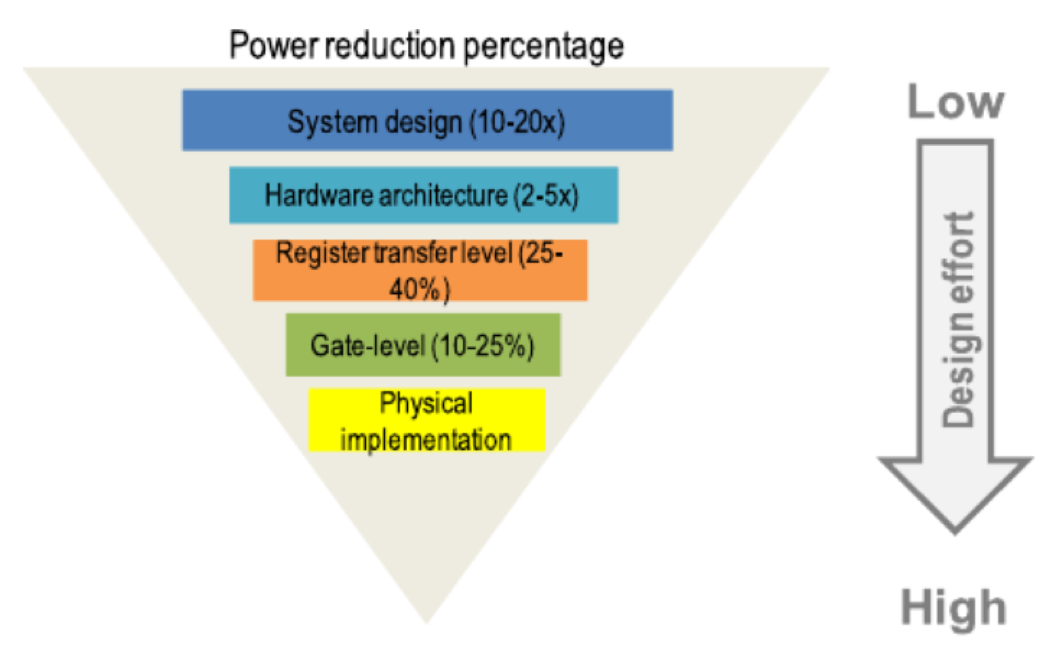
\includegraphics[scale=.4]{Picture1.png} 
\caption{Potential power savings at various levels of abstraction}
\end{figure}

\section{Contributions}
Our contribution is to automate the design space exploration of HLS projects. We have developed and efficient method that allows Cruise Control to produce a valid solution. To reach this goal, our parser would be developed from scratch. The syntax that it will be looking for is native to HLS applications and can be accomplished  with regular expression processing. We will also have to define and model our own search algorithm for the state space which is something that is also unique. Our approach uses both breadth first search (BFS) as well as random sampling to reach a solution.  Finally, we will have to write our own tool command line (TCL) scripts to automate the process and handle the integration with Vivado HLS. This script was also developed from scratch and is used to make Cruise Control as simple as possible for designers. We believe that these contributions are unique and can make an impact on the HLS community. All of the code is open source and can be found on the Cruise Control Git Hub [X]. 


\section{Approach}
Our approach to create Cruise Control can be broken up into a few steps outlined in Figure 2. The first step in the control flow is to preform pre-processing on the input C or C++ file.  The pre-processing includes scanning the input file for for loops. The pre-processor then enters two lines after each instance of a for loop. This is done because the second part of the input parser needs to have these spaces to input the pragmas automatically. The pre-processor outputs a template file with the added spaces for the second part of the input parser to use. The parser was aided by the regex library and run on a Linux machine.  \newline

\begin{figure}[H]
\centering
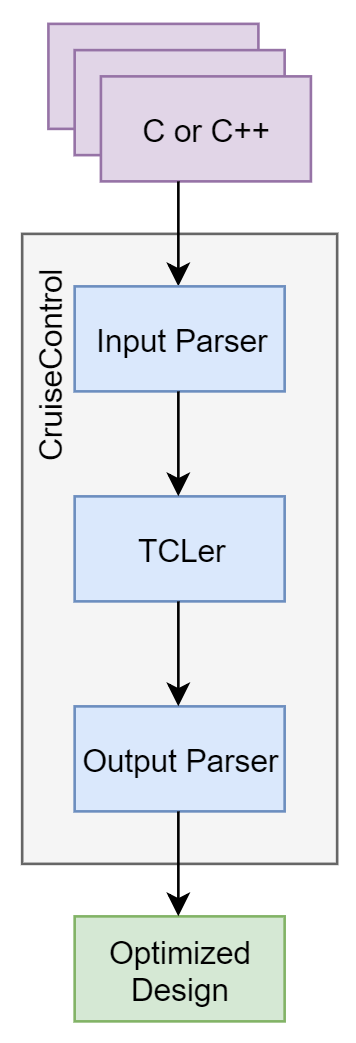
\includegraphics[scale=.6]{CC_flow.png} 
\caption{Cruise Control  flow}
\end{figure}

After the lines have been added to the input file, the second step of the input parser begins. This portion of the input parser finds the for loops once again and automatically inserts the pragmas. The choice to include the pragma is seen as a binary decision in Cruise Control. The pragma is either placed or is not placed. With this in mind, the state space of Cruise Control can be defined by a set of binary numbers. Each for loop in the source code is given an index into the binary number and each index has a value corresponding to if the pragma is placed or not placed. This allows Cruise Control to have a finite set of states to explore. Figure 3 shows an example of what a nested for loop structure will become after the input parser processes it. \newline

\begin{figure}[H]
\centering
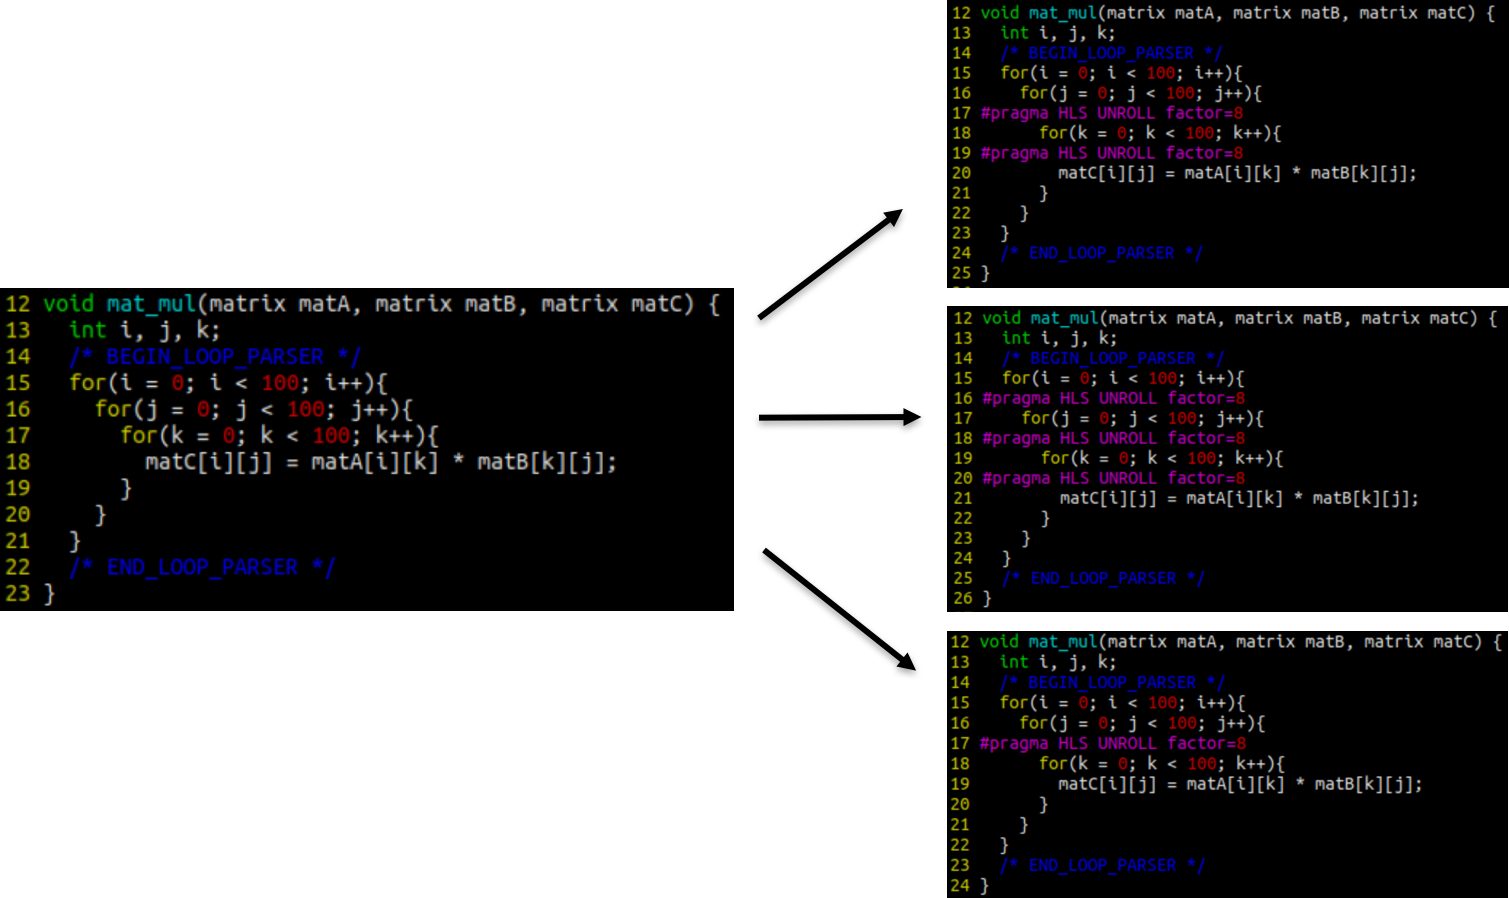
\includegraphics[scale=.35]{for_loops.png} 
\caption{Loop nesting processing}
\end{figure}

The input parser works by cycling through all possible design states and entering the pragmas in unique patterns. The parser then saves these files with the binary number corresponding to the pragma placement appended to the end. All of the different files are saved into a folder for easy access. The input parser also creates a text file with the total number of states created as well as each state space file name. The text file with the number of runs and file names is the input into the  TCL script that controls the second part of Cruise Control.  \newline

The TCLer is the second step in Cruise Control. Figure 4 outlines the design flow for this portion of the tool. The TCLer is a TCL script that takes in the folder of design space enumerations as well as the text file generated by the input parser. The top of the text file stores the integer number of how many runs must be synthesized and analyzed. The script automatically reads in this value when invoked. There is set up required by the user to allow the script to run correctly for each HLS project. This includes naming the project, the top level function, a test bench file, and any other library files. If these files are not in the project directory the script fails. There are also lines to change the targeted device and clock speed for the design. After the user enters the file names, the script can be invoked from within the project directory. Cruise Control expects to be run from inside a preexisting HLS project.  The script also expects the design space files to be copied into the main directory of the project. \newline

The script is run through the command line interface on a Windows machine. The script works by looking for the design space file listed in the text file. After this file is found, the script creates a solution and begins to synthesize the project according to the pragmas listed in the design space file. After the synthesize is complete, the script opens the solution file and copies the latency report to a report file. This report file is used by the output parser to find the design space state that creates the optimal solution. As the TCLer runs, it deletes the design space files so the project directory remains uncluttered with test files. 


\begin{figure}[H]
\centering
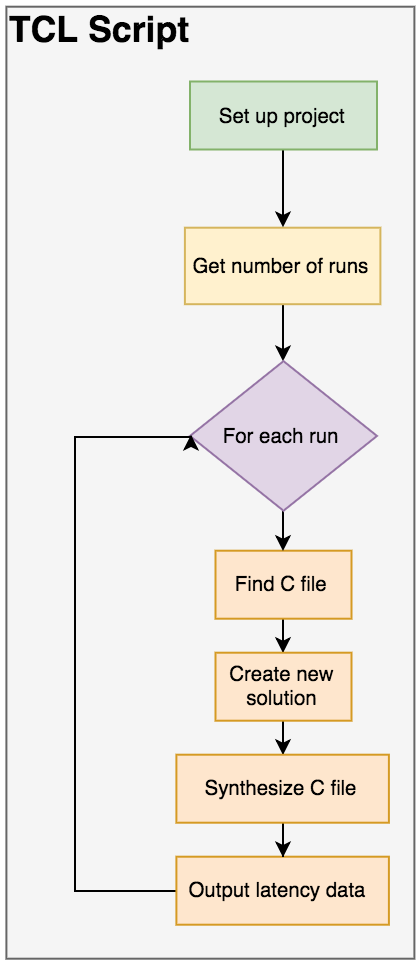
\includegraphics[scale=.5]{tcler.png} 
\caption{TCLer control flow}
\end{figure}

The output of the TCLer is a report file that contains the latency numbers for each design iteration. An example of the output format is shown in Figure 5. The output parser accepts this report file as an input. With the report file, the output parser is able to isolate the exact cycle latency for each design. The latency count and iteration number are formatted and exported to a text file which allows the information to be easily copied into and Excel sheet. Within the Excel sheet, the user can find the design space state that fits their desired speed up.


\begin{figure}[H]
\centering
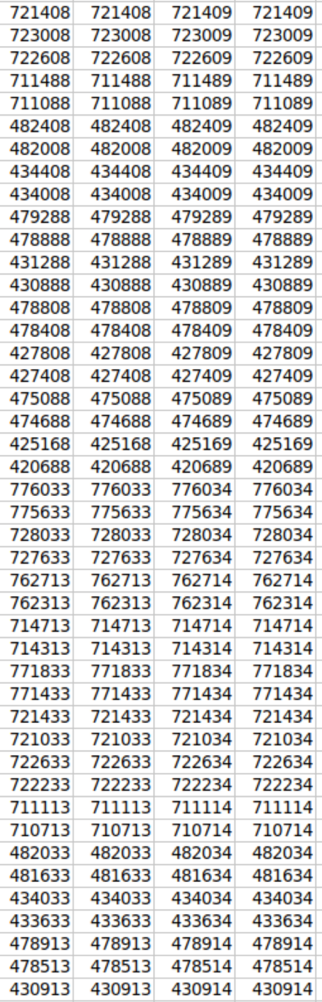
\includegraphics[scale=.5]{outputparser.png} 
\caption{Output parser format}
\end{figure}

\section{Experiment}
To gather data on Cruise Control's performance, different HLS projects were tested. First, a simple matrix multiplication was used to verify that Cruise Control can create the correct design space files and synthesize different runs automatically. The output report file from the matrix multiplication was also used to examine the output parser to see if Cruise Control can isolate the output latency. The matrix multiplication file had a triple nested for loop which correlates to eight design space states. \newline 

After the functionality of Cruise Control was verified, a larger HLS project was used to analyze how well Cruise Control can scale and perform on larger projects. The larger project used was a the fifth convolution layer from LeNet. This file had several nested for loops which resulted in 128 design space states to explore. This was a familiar implementation due to previous assignment in the class as well so working with the project was easy. For the larger projcts Cruise Control analyzed all 128 states and produced the report file to be analyzed once again. The process was repeated for the fully connected layer of LeNet as well. This implementation also had 128 design state spaces to enumerate.  


\section{Results}
With the output report files from Cruise Control, results of the performance were easy to obtain. Figure 6 shows the max speed up found by Cruise Control for both the large and small tests. 

\begin{figure}[H]
\centering
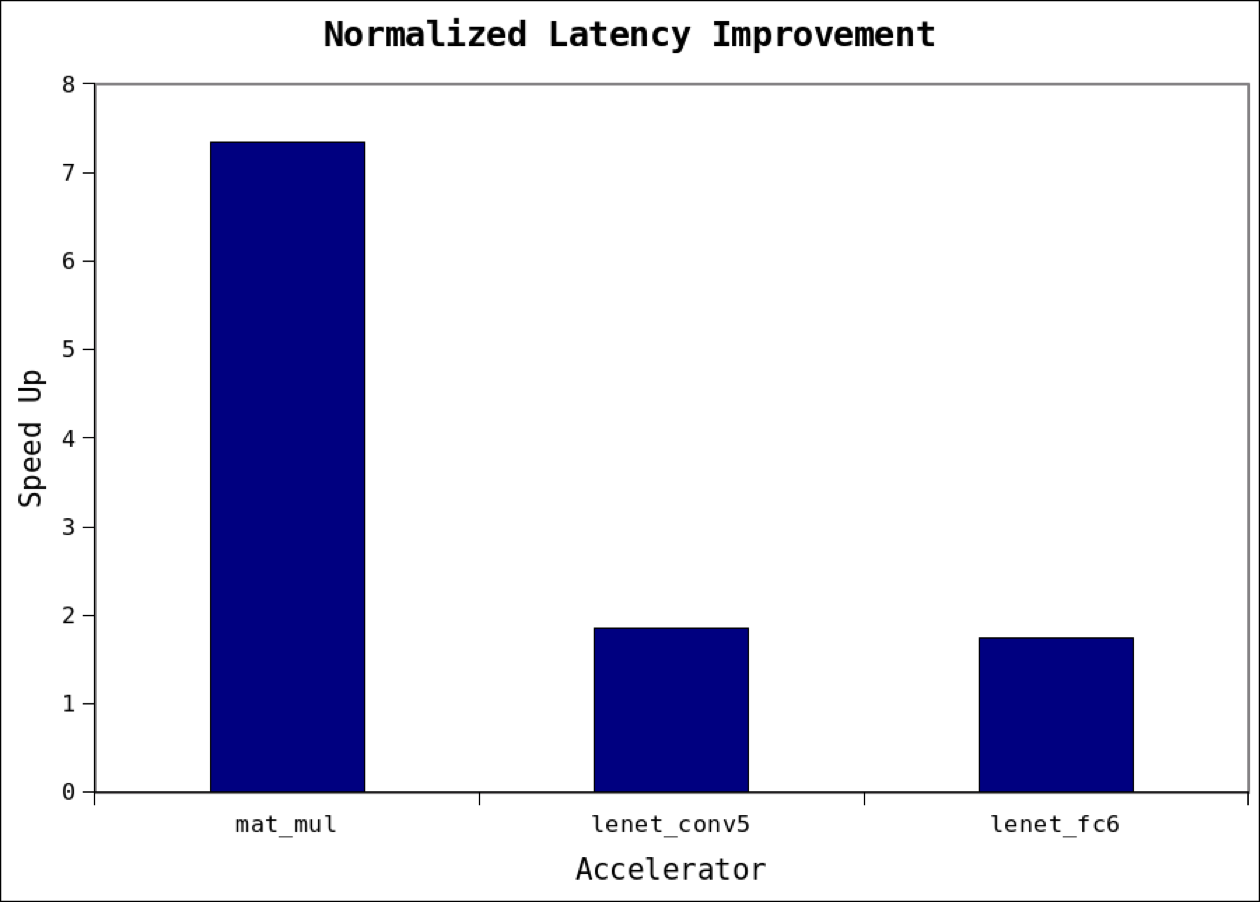
\includegraphics[scale=.4]{result0.png} 
\caption{Cruise Control performnace speed ups}
\end{figure}

The itemized list of run iteration and cycle count could be easily graphed. The first run that Cruise Control analyzes is the original source code without any pragmas inserted. This allows performance numbers to be generated to see speed up from the original design. Figure 7 shows the data collected from the matrix multiplication test. The first few run iterations had little effect on the performance of the design. The last few iterations evaluated showed a 7.5x speed up from the base design. This result shows that Cruise Control is able to discover and leverage the inherit speed up found in parallel work. \newline 

\begin{figure}[H]
\centering
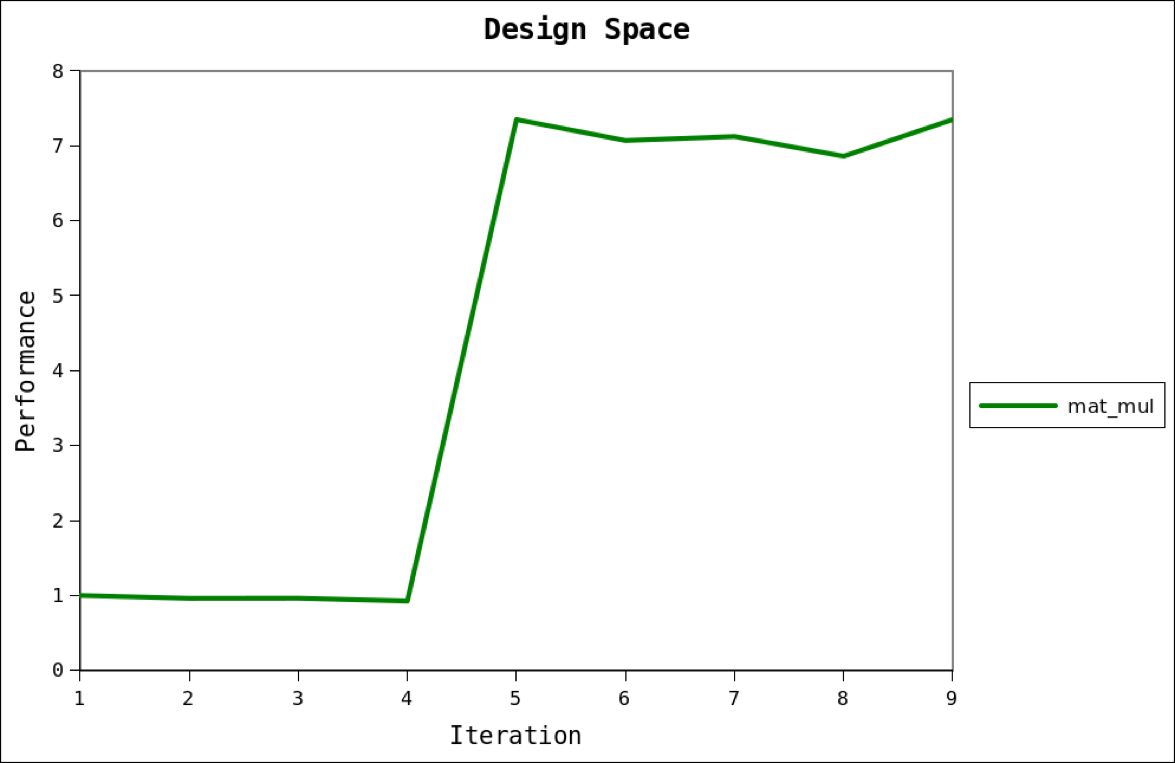
\includegraphics[scale=.45]{result1.png} 
\caption{Matrix multiplication results}
\end{figure}

When looking at larger designs, more conclusions can be reached. Figure 8 outlines the results found for the larger tests of Cruise Control on the fifth convolution layer and fully connected layers for LeNet. As these results show, there are a few design states that have significant negative impacts on the performance. This is because of the loop unroll factor chosen for the parallel work did not always match the bounds of the for loops. This design choice produces more dense logic that becomes a bottle neck for the design as opposed to accelerating it. Significant performance increases were also discovered in the search by Cruise Control. States that resulted in a 1.8x speed up for both tests were found. The wave like data shown in the graph comes from the similarity in variations of the pragma placement. Often, the choice to include or exclude the pragmas in different locations can have identical impacts on performance. \newline

\begin{figure}[H]
\centering
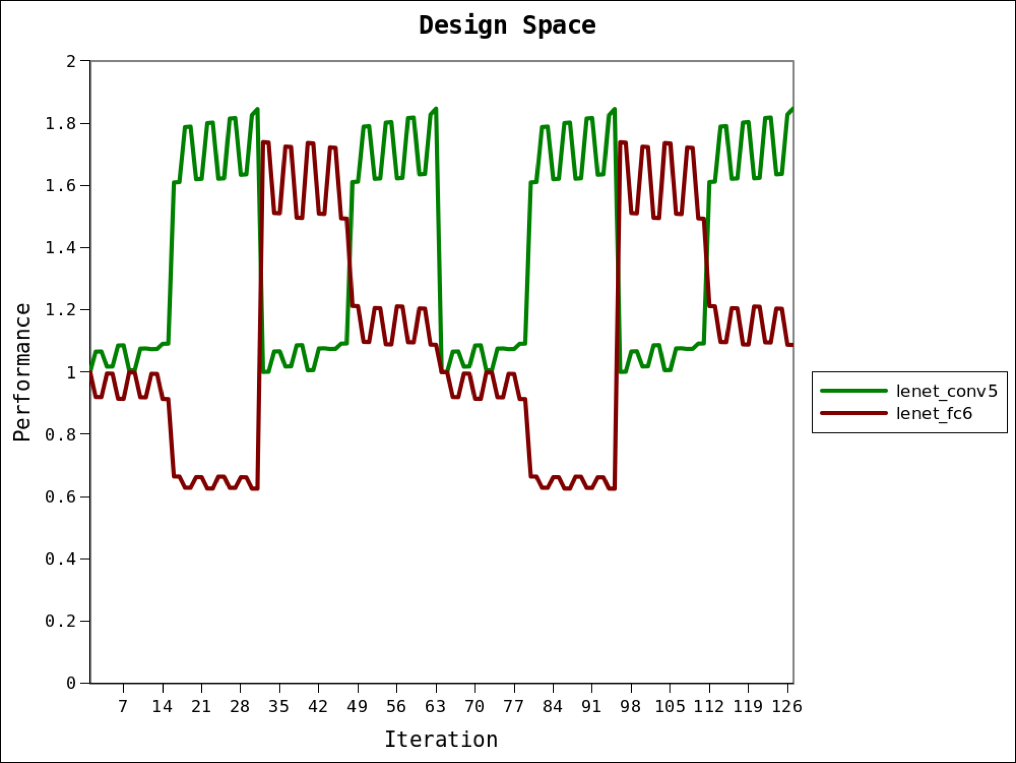
\includegraphics[scale=.45]{result2.png} 
\caption{LeNet layer results}
\end{figure}


In addition to the performance speed up found by Cruise Control, the automation aspects of the tool are able to save designers significant time while developing HLS project. A few students familiar with the design flow for HLS projects were asked to manually examine the code for the fifth convolution layer in LeNet. All students had seem this code before and understand how the convolution layers function. The students were timed as they entered pragmas and synthesized the design on their own. After each synthesis, the students manually checked the reports to see their design speed ups. The students worked until they found a design that was similar to the solution found by Cruise Control. It was found that each students takes on average 5.4 minutes to complete a single design iteration manually. Cruise Control was able to evaluate a design state for the fifth convolution layer in about 21 seconds. This is about a 15.5x speed that the designer can leverage. As Cruise Control runs, the user can also work on other features in the design. This speed up was a significant contribution to the capabilities of Cruise Control. 



\section{Conclusion}
In this paper we present Cruise Control, an automatic tool to explore the design space for HLS projects. The control flow for the project is broken into an input parser to pre-process the input design, a TCL script to automate the design state exploration, and and output parser to format the results for easy examination. As seen from the results, Cruise Control is able to properly find a valid design state that optimizes the performance of a HLS design. From small to large projects, Cruise Control quickly moves through the search states to find a solution. In addition to the performance increases, Cruise Control is able to perform its jobs much more quickly than a human designer. This time saved can be of great use because now the designer can work on other material as Cruise Control runs knowing an optimal solution will be produced. The tool is also easy to integrate into any existing  HLS project. The tool is in early stages of the design process and can be capable of much more. 


\section{Future Work}
There is some work that can be done on Cruise Control. One of the most important works to be done is a smarter design space search algorithm. A BFS is currently used which can result in long run times for the tool. As the number of for loops increases in a design, the total number of states increase exponentially. This exponential growth is not good. To counter this issue, a heuristic base search can be implemented to cut down the number of states explored. Only pursing states that have a high probability of being optimal would make the scaling more efficient. \newline
Adding support for power analysis would also allow Cruise Control to factor in power constraints on designs. To have a power report though, the placement and routing for the HLS project must be run. This run is often time consuming and would render the time saving ability of Cruise Control useless. If there was an approximation engine for the HLS project that could help save some time in this area and would add a core functionality to the tool. \newline
Lastly, different optimization pragmas can be tried as well. The current tool only looks for for loops to add loop unrolls. Other pragmas such as pipelines and interfaces can also be added to the design to reach even larger performance increases for the design. 


\section{Cited Works}
\noindent [1] Xilinx Vivado HLS \\
\noindent [2] J. Cong, B. Liu, S. Neuendorffer, J. Noguera, K. Vissers, and
Z. Zhang. High-level synthesis for fpgas: From prototyping
to deployment. Trans. Comp.-Aided Des. Integ. Cir. Sys.,
30(4):473–491, Apr. 2011.\\
\noindent [3] A. Qamar, F. Muslim, J. Iqdal, and L. Lavagno, LP-HLS: Automatic Power-Intent Generation for High-Level Synthesis Based Hardware Implementation Flow. Microprocessors and Microsystems. 50. 10.1016/j.micpro.2017.02.002.  \\
\noindent [4] atsmith3 - https://github.com/atsmith3/CruiseControl





\end{document}